\section{Physics Informed Neural Networks}
\label{sec:literature-review-physics-informed-neural-network}

Applications of deep learning methods have been achieving multiple breakthroughs, especially in computer vision and natural language processing.
The performance of these models is enabled by utilizing a vast amount of data that is readily available.
Nonetheless, the application of deep learning in many domains of science has not been gaining success.
The cost of data collection for analyzing complex physical, biological, or engineering systems is prohibitive.
Without big data, state-of-the-art deep learning techniques lack robustness and are not guaranteed to converge.
Specifically, in the case of Covid-19 or any other disease, an accurate model, that can fairly estimate the trajectories of the disease at an early stage when data is scarce, is highly desirable.
Prior knowledge about dynamical systems, which is captured by mechanistic models, had not been utilized for training \glspl{ANN} \cite{raissiPhysicsinformedNeuralNetworks2019}.
By utilizing this information, the solutions space that an \gls{ANN} can take can be limited and the data seen by models is enriched to help them converge faster.
\glspl{PINN} work by using the knowledge given by mechanistic models in the form of \glspl{ODE} or \glspl{PDE} as a regularization term for the loss function \cite{raissiPhysicsinformedNeuralNetworks2019, lagarisArtificialNeuralNetworks1998}.
With physical constraint incorporated within the loss function, the \glspl{ANN} is guided to learn the parameters that give rise to a solution that obeys physical laws.
\autoref{fig:pinn-schematic} shows the general schematic of \glspl{PINN}.

To derive the loss function for \glspl{ODE} in this framework, first the following equation is considered \cite{lagarisArtificialNeuralNetworks1998}
\begin{equation}
    \frac{du}{dt} = f(u, t),\ t \in [0, 1],\ u(0) = u_0
\end{equation}
An \gls{ANN} is then used to approximate the solution to this problem
\begin{equation}
    \mathcal{NN}(t) \approx u(t).
\end{equation}
Because the \gls{ANN} is differentiable and assuming that $\mathcal{NN}(t)$ is the solution of the problem, then $d\mathcal{NN}(t)/dt = f(\mathcal(NN)(t), t)$ for all $t$.
This condition can then be incorporated into the loss function
\begin{equation}
    MSE = \frac{1}{N} \sum_i^N \left( \frac{d\mathcal{NN}(t_i)}{dt} - f(\mathcal{NN}(t_i), t_i) \right)^2.
\end{equation}
Note that the initial condition $u(0) = u_0$ has to be satisfied.
Thus a new function is defined that encodes the initial condition within itself. This function will trivially satisfies the initial condition for any possible set of parameters
\begin{equation}
    g(t) = u_0 + t\mathcal{NN}(t).
\end{equation}
The function above inherits the property of \glspl{ANN} as universal approximators for any continuous function while satisfies the condition $g(0) = u_0$.
At this point, the loss function turns into
\begin{equation}
    MSE = \frac{1}{N} \sum_i^N \left( \frac{dg(t_i)}{dt} - f(g(t_i), t_i) \right)^2.
\end{equation}

\begin{figure}[h]
    \centering
    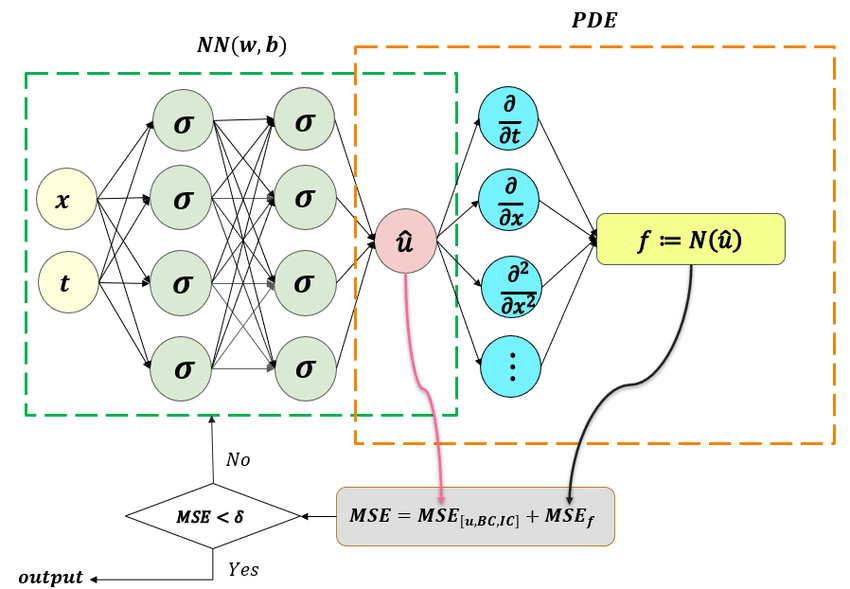
\includegraphics[scale=0.3]{pinn-schematic.png}
    \caption{The schematic of PINNs for solving PDEs. Figure is taken from \cite{guoSolvingPartialDifferential2020}}
    \label{fig:pinn-schematic}
\end{figure}

To derive the loss function for \glspl{PDE} in this framework, the parameterized nonlinear \glspl{PDE} of the general form is first considered \cite{raissiPhysicsinformedNeuralNetworks2019}
\begin{equation}
    u_t + \mathcal{N}[u; \lambda] = 0,\ x \in \Omega,\ t \in [0, T],
    \label{eq:pinn-general-pde}
\end{equation}
where $u(t, x)$ denotes the hidden solution, $\mathcal{N}[\cdot; \lambda]$ is a nonlinear differential operator parameterized by $\lambda$, and $\Omega$ is a subset of $\mathbb{R}^D$.
The function $f(t, x)$ is defined to be given by the left-hand side of \autoref{eq:pinn-general-pde}
\begin{equation}
    f := u_t + \mathcal{N}[u].
    \label{eq:pinn-pde-condition}
\end{equation}
The hidden solution $u(t, x)$ is then approximated by an \gls{ANN}, denoted as $\hat{u}(t, x) = \mathcal{NN}(t, x)$.
From the approximation $\hat{u}(t, x)$ and \autoref{eq:pinn-pde-condition}, the function $\hat{f}(t, x)$ can be defined that describes the \glspl{PDE} in terms of the approximation
\begin{equation}
    \hat{f} := \hat{u}_t + \mathcal{N}[\hat{u}].
\end{equation}
To train the parameters of the \gls{ANN}, the following loss function is employed \cite{raissiPhysicsinformedNeuralNetworks2019}
\begin{equation}
    MSE = MSE_u + MSE_f,
\end{equation}
where
\begin{equation}
    MSE_u = \frac{1}{N_u} \sum_{i=1}^{N_u} |\hat{u}(t_u^i, x_u^i) - u^i|^2
\end{equation}
and
\begin{equation}
    MSE_f = \frac{1}{N_f} \sum_{i=1}^{N_f} |\hat{f}(t_f^i, x_f^i)|^2.
\end{equation}
$\{t_u^i, x_u^i, u^i\}_{i=1}^{N_u}$ are the initial and boundary training data, and $\{t_f^i, x_f^i\}_{i=1}^{N_u}$ are the collocation points.
The loss value $MSE_u$ enforces the initial and boundary conditions on the \gls{ANN}, while the loss value $MSE_f$ enforces the dynamics specified by \autoref{eq:pinn-general-pde}.

The \gls{ANN} under this framework can be training using well-known techniques in deep learning.
These techniques include automatic differentiation, back-propagation, and gradient-based optimization.
Empirical evidence showed that the \gls{ANN} will converge to a global minimum under the condition that the differential equations are well-posed and their solution is unique \cite{raissiPhysicsinformedNeuralNetworks2019}.
They also showed that the model achieved high prediction accuracy with out-of-sampled data when given a sufficiently expressive \gls{ANN} and a sufficient number of collocation points $N_f$.